\documentclass{article}
\usepackage{graphicx}
\usepackage{amsfonts}
\usepackage{amsmath}
\usepackage{amssymb}
\usepackage{tikz}


\title{Definition for Mathematical Expression for Computer Science}
\author{Sarah Liu}
\date{January 2026}

\begin{document}

\maketitle

\section{Basic Logic}
\subsection{Necessary Conditions, and Sufficient Conditions}
Let $C$ and $N$ be conditions. Then $N$ is \textbf{necessary} for $C$ means: whenever $C$ is true, $N$ must be true.

Let $C$ and $S$ be conditions. Condition $S$ is \textbf{sufficient} for condition $C$ means: whenever $S$ is true, $C$ must be true.


\subsection{Universal and Existential Quantification}

These are called \textbf{universal quantification} and \textbf{existential quantification}.
The parameters of these notations are:
\begin{itemize}
    \item a variable name v (called the \textbf{quantified variable})
    \item a set D (called the \textbf{domain})
    \item a boolean expression e (called the \textbf{body}), which may (and usually does) involve the variable name
\end{itemize}


\subsection{Predicates}

A function that produces booleans is called a \textbf{predicate}. We can write
\[
P:D\rightarrow\mathbb{B}
\]
to specify that $P$ is a \textbf{unary} (i.e., one-parameter) predicate with \textbf{domain} $D$. We can also say this as: $P$ is a predicate \textbf{on} $D$, or $P$ is a predicate \textbf{over} $D$.


\subsection{Exploring Logical Forms}
For conditions $C$ and $C'$ about $P$, $C$ \textbf{entails} $C'$ means: whenever $C$ is true for $P$, then $C'$ is true for $P$.\footnote{This is the same as $C$ being sufficient for $C'$, and also the same as $C'$ being necessary for $C$, but is simpler to write and say.}

\subsection{Universally Quantified Implication}
A \textbf{universally quantified implication} is a special form of \textit{universal} quantification, used to express a \textbf{restriction of the domain}
using a special form of body:
\[
\forall v\in D, (r\rightarrow e)\text{ means }\forall v \in \{v\in D: r\}, e
\]
The additional parameters of this notation are:
\begin{itemize}
\item a condition r (called the \textbf{antecedent})
\item a condition e (called the \textbf{consequent})
\end{itemize}
We’ll also refer to r as a \textbf{precondition} or \textbf{restriction} on v.

\subsection{Existentially Quantified Conjunction}
In general, \textit{for an existential}, conjoining a condition in the body \textit{has the effect} of \textbf{restricting the domain}:
\[
\exists v\in \{v\in \mathcal{D}:p\},q \equiv \exists v\in \mathcal{D},(p\wedge q)\equiv \exists v\in \mathcal{D},(q\wedge p) \equiv \exists v\in \{v\in \mathcal{D}:q\},p
\]\footnote{Note that because the relation holds for existential quantifier, it also holds for universal quantifier.}

\subsection{Contrapositives}

If $\mathcal{P} \subset \mathcal{Q}$ then if an element is not in $\mathcal{Q}$ then it’s not in $\mathcal{P}$ — and conversely. So:
\[
\forall v\in\mathcal{D},P(v)\rightarrow Q(v) \equiv \forall v\in\mathcal{D},\neg Q(v)\rightarrow\neg P(v)
\]
These are called each other’s \textbf{contrapositives}.

\subsection{Biconditionals}
For a variable name v, domain set D, and conditions p and q, we define
\[
\forall v \in D, (p \leftrightarrow q) \quad\text{to mean} \quad (\forall v \in D, p \rightarrow q) \wedge (\forall v \in D, q \rightarrow p) .
\]

The symbol $\leftrightarrow$ is called the \textbf{biconditional}, often read as “iff”.

So a standard direct proof of $\forall v \in D, (p \leftrightarrow q)$ would prove each conjunct (each \textbf{direction} of the biconditional).


\newpage
\section{Runtime}

For $f:N \rightarrow R$ and $g:N \rightarrow R$, we define $g$ \textbf{eventually dominates} $f$ to mean:
\[
\exists n_0\in\mathbb{N},\; \forall n\in \mathbb{N}, \; n\geq n_0\rightarrow g(n)\geq f(n)
\]

\subsection{$\omega$}


\subsection{Big-O and Big-$\Theta$}

For $f,g$ eventually defined, define $f$ \textbf{is Big-O of} $g$, written symbolically as $f\in\mathcal{O}(g)$, to mean
\[
\exists c\in\mathbb{R}^+,\text{eventually}\; f\leq c\cdot g\equiv\exists c\in\mathbb{R}^+,\exists n_0\in \mathbb{N}, n\geq n_0\rightarrow f(n)\leq c\cdot g(n)
\]

For $f,g$ eventually defined, define $f$ \textbf{is Big-$\Theta$ of} $g$, written symbolically as $f\in\mathcal{\Theta}(g)$, to mean
\[
f\in\mathcal{O}(g) \wedge g\in\mathcal{O}(f)
\]

\subsection{Ceiling and Floor}

Let $x \in \mathbb{R}$. The \textbf{ceiling} of $x$, written symbolically as $\lceil x \rceil$, is the smallest integer that is at least as large as $x$:
\[
\lceil x \rceil = \min\{ z \in \mathbb{Z} : x \le z \}.
\]

Similarly, the \textbf{floor} of $x$, written symbolically as $\lfloor x \rfloor$, is the largest integer that is no more than $x$:
\[
\lfloor x \rfloor = \max\{ z \in \mathbb{Z} : z \le x \}.
\]

\newpage
\section{Additional Comment}
\subsection{Mechanical Substitution}
In this course, we will discuss the set of \textbf{natural numbers} unless specified otherwise. Note that $\mathbb{N} = \{0,1,2,3,\dots\}$, \textit{which includes zero}.

The first variable dealt in the problem is $n$, \textbf{declared} with the \textbf{precondition} that it’s a natural
number. This precondition is naturally expressible as being in a standard set, i.e., as $n \in N$, which we call the variable’s domain.

To see if the variable behaves as a parameter we \textbf{instantiate} the problem with a value (that satisfies the precondition, i.e., is in
the domain) for the variable. So we take a specific natural number and \textbf{syntactically} (i.e., textually) substitute (i.e., replace) the
variable name with the value, in the body of the problem (which is the part of the problem text without the declaration of the
parameter)\footnote{The process of \textit{mechanical substitution} is used throughout this course.}

Coming up with good examples when problem-solving is similar to coming up with \textbf{good test cases} in Software Engineering. And Test-Driven Development recognizes that test cases are more than just for testing: developing test cases is valuable to also
\textit{understand, solve, and document} a problem. Tests cases are often classifed as \textbf{edge/boundary/special/extreme/corner} versus \textbf{generic/typical/representative}.

\subsection{Conjunction and Disjunction}
Combining two conditions into one condition that expresses that both conditions are true is called \textbf{conjunction}. Symbolically, we use the binary conjunction operator “$\wedge$”. The combined expression is called a \textbf{conjunction}, and the conditions being combined are called \textbf{conjuncts}.\footnote{People often refer to the symbol $\wedge$ as “and”, but it is \textit{not} simply an abbreviation of that word. The symbol is used \textit{only} for
conjunction, which combines \textit{only} true/false (aka boolean) expressions (aka \textbf{propositions}) to construct a claim that both are true.}

Combining two conditions into one condition that expresses that \textit{at least one} (i.e., \textit{one or both}) of two conditions is true is called
\textbf{disjunction}. Symbolically, we use the binary disjunction operator “$\vee$”. This operation is sometimes referred to as “\textbf{inclusive}
or”, and the symbol $\vee$ referred to as “or”.
So, for example, we can write the solution of the previous activity as: $a \geq 1 \vee b \geq 1$. The combined expression is called a
\textbf{disjunction}, and the conditions being combined are called \textbf{disjuncts}.

\subsection{Universal and Existential Quantification}
People sometimes refer to the symbols $\forall$ and $\exists$ as “for all” and “there exists”, but these symbols are \textit{not} simply abbreviations of
English words / phrases. In fact, we do not give them a meaning on their own.
The above \textit{expression forms} have meanings, which are the following expansions:
\[
\begin{aligned}
\forall v \in \{x_0, x_1, x_2, \ldots\},\ e &\text{ means }
e_{x_0} \wedge e_{x_1} \wedge e_{x_2} \wedge \cdots \\
\text{and }\quad\exists v \in \{x_0, x_1, x_2, \ldots\},\ e &\text{ means }
e_{x_0} \vee e_{x_1} \vee e_{x_2} \vee \cdots
\end{aligned}
\]

\subsection{Graphic Representation of Set Relations}
A \textbf{Venn diagram} for sets draws the sets as intersecting circles, so that every \textit{potential} containment and overlap can be considered.

An \textbf{Euler diagram} shows a specific relationship between sets.

The following shows:
\begin{itemize}
\item a Venn diagram for $\mathcal{D}$ and $\mathcal{O}$
\item an Euler diagram showing the claim that $\forall n\in \mathcal{D}$, n is odd, i.e., that each element of $\mathcal{D}$ is odd
\item the Venn diagram with the element 2 showing that the claim is false
\end{itemize}

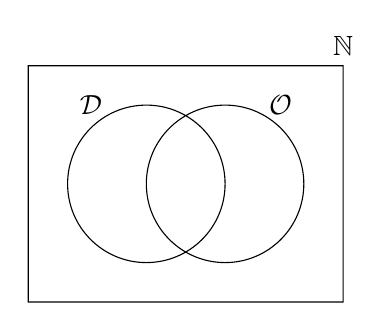
\begin{tikzpicture}
\draw (0,0) circle (1) (0,1)  node [text=black,xshift=-20pt] {$\mathcal{D}$}
      (1,0) circle (1) (1,1)  node [text=black,xshift=20pt] {$\mathcal{O}$}
      (-1.5,-1.5) rectangle (2.5,1.5) node [text=black,above] {$\mathbb{N}$};
\end{tikzpicture}

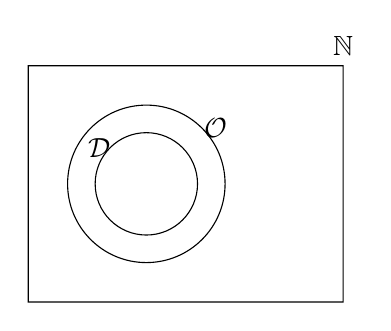
\begin{tikzpicture}
\draw (0,0) circle (1) (0,0)  node [text=black,xshift=-17pt,yshift=13pt] {$\mathcal{D}$}
      (0,0) circle (0.65) (0,0)  node [text=black,xshift=25pt,yshift=20pt] {$\mathcal{O}$}
      (-1.5,-1.5) rectangle (2.5,1.5) node [text=black,above] {$\mathbb{N}$};
\end{tikzpicture}


\subsection{False Statement for Conjunction and Disjunction}
A single true disjunct is enough to show that a \textit{disjunction is true}, so a single instance of the body of \textit{an existential} (an existentially quantified statement) is enough to show that the existential is true. We say that the element of the domain
which produces that instance of the body is a \textbf{witness} to/for the existential (being true). We can also describe this in terms of the body as: the instance of the body \textbf{witnesses} (the truth of) the existential.

A single false conjunct is enough to show that a \textit{conjunction is false}, so a single instance of the body of \textit{a universal} (a universally quantified statement) is enough to show that the universal is false. We say that the element of the domain which produces that instance of the body is a \textbf{counter-example} to / for the universal. We can also describe this in terms of the body as: the instance
of the body being false \textbf{counters} (the truth of) the universal.

\subsection{Relationship for Conjunction$\backslash$Disjunction and Necessary$\backslash$Sufficient}
A useful relationship between conjunction and necessity, and between disjunction and sufficiency is as follows:

If C is equivalent to a conjunction containing N as a conjunct, then N is necessary for C.

If C is equivalent to a disjunction containing S as a disjunct, then S is sufficient for C.

\subsection{Equivalence}
When two expressions produce the same boolean value, we say they are \textbf{equivalent}, which is written symbolically as “ $\equiv$ ”.

The $\equiv$ operator and its negation $\not\equiv$ have lower precedence than \textit{every} operator in this course. For example, $p \wedge q \equiv r$ is interpreted as $(p \wedge q) \equiv r$.


\footnote{Whenever predicate is true for all number, then the existential is true.}

\subsection{Exploring Logical Forms}
Illustrated table are a good way to visualize predicates.

\subsection{Negation}
\textbf{Negation} is the operation that claims a condition is false. It’s written symbolically as “$\neg$”, which is a \textbf{unary prefix} operator, and is often read as “not”.

The operator $\neg$ has \textit{higher precedence} than $\wedge$ and $\vee$: in an expression with these it applies to the first complete boolean sub-expression to the right of it.

\subsubsection{Negated Quantification}
In general:
\[
\begin{aligned}
\neg \forall v\in \mathcal{U}, \mathcal{Q}(v) &\equiv\exists v\in\mathcal{U},\neg \mathcal{Q}(v)\\
\neg \exists v\in \mathcal{U}, \mathcal{Q}(v) &\equiv\forall v\in\mathcal{U},\neg \mathcal{Q}(v)
\end{aligned}
\]

These, along with $\neg\neg p\equiv p$, represent the reasoning about the equivalences in the negation.

\subsubsection{Negated Conjunction and Disjunction}
Since quantification is just repeated conjunction or disjunction, we can say something analogous about negations of explicit conjunctions and disjunctions.

\[
\begin{aligned}
    \neg \forall v\in\{v_0,v_1,\dots\},R(v) &\equiv \exists v\in\{v_0,v_1,\dots\},\neg R(v)\\
    \neg (R(v_0)\wedge R(v_1)\wedge\dots) &\equiv \neg R(v_0)\vee \neg R(v_1)\vee\dots
\end{aligned}
\]
In particular for conditions $p$ and $q$:
\[
\neg (p\wedge q) \equiv \neg p\vee \neg q
\]
In other words: if it isn’t the case that both $p$ and $q$ are true, then at least one is false.

\[
\begin{aligned}
    \neg \exists v\in\{v_0,v_1,\dots\},R(v) &\equiv \forall v\in\{v_0,v_1,\dots\},\neg R(v)\\
    \neg (R(v_0)\vee R(v_1)\vee\dots) &\equiv \neg R(v_0)\wedge \neg R(v_1)\wedge\dots
\end{aligned}
\]

In particular for conditions $p$ and $q$:
\[
\neg (p\vee q) \equiv \neg p\wedge \neg q
\]

In other words: if it isn’t the case that at least one of $p$ and $q$ is true, then both are false.


\subsection{Nested Quantification}
There’s a shorthand notation for nested quantification of the same kind with the same domain:

\[
\begin{aligned}
\forall v_0, v_1, \ldots, v_n \in D,\ e &\text{ means } \forall v_0 \in D, \forall v_1 \in D, \ldots, \forall v_n \in D,\ e \\
\exists v_0, v_1, \ldots, v_n \in D,\ e &\text{ means } \exists v_0 \in D, \exists v_1 \in D, \ldots, \exists v_n \in D,\ e
\end{aligned}
\]


\subsection{Proof}
A \textbf{direct proof} is a proof “directly” followed the logical structure of the statement.

Prove this statement:

\[
\forall a,b \in \mathbb{N},\ (a \ge 1 \wedge b \ge 1 \wedge (a \ge 2 \vee b \ge 2) 
\;\rightarrow\; a \cdot b \ge 2)
\]

Let $a,b \in \mathbb{N}$. 

Suppose $a \ge 1$, and $b \ge 1$, and $a \ge 2$ or $b \ge 2$. 

Case $a \ge 2$: 

\qquad Then $a \cdot b \ge 2 \cdot 1 = 2$. 

Case $b \ge 2$: 

\qquad Then $a \cdot b \ge 1 \cdot 2 = 2$. 

For universal statements, the proof first declared the universally quantified variables with their domains, as parameters of
the proof. 
In this course, to declare a variable, we write: “Let $v_0,\dots, v_n \in D$.”.

For existential statements, we need to instantiate the case that we are proving. In this course, we use the phrase: “Set $v=\_\_\_$.”

For universally quantified implication, we then assumed the antecedent. Two common phrasings of an assumption
are “Suppose ...”, and “Assume ...”.

When we assume a conjunction, we assume each conjunct. Technically, when we wrote “Suppose $a \geq 1$, and $b \geq 1$,
and $a \geq 2$ or $b \geq 2$”, we meant “Suppose $a \geq 1$, and suppose $b \geq 1$, and suppose $a \geq 2$ or $b \geq 2$”.\footnote{Don’t use “$\wedge$” here: we don’t express \textit{logical
structure} symbolically in “real” proofs.}

Because one of the three assumptions was a disjunction, we proceeded by proving the consequent by cases, based on the disjuncts.

Prove:
\[
\exists n \in N, \;\forall k \in N,\; k \geq n \rightarrow k^3 - 3k \text{ is composite.}
\]

Set $n=3\in \mathbb{N}$.

Let $k\in\mathbb{N}$.

Assume $k\geq n=3$.

Then $k>1$.

And $k^2-3\geq 3^2-3=6>1$.

And $k^2-3\in\mathbb{N}$, since $k^2-3\in\mathbb{Z}$ and $k^2-3>1$.

And $k^3-3k=k\cdot (k^2-3)$.

So $k$ and $k^2-3$ are witnesses that $k^3-3k$ is composite.

Prove:
\[
\forall n \in N, \;\exists k \in N,\; k \geq  n \wedge k^3 - 3k \text{ is composite.}
\]

Let $n \in N$.

Set $k = \max(3,n) \in N$.

Then $k \geq n$.

And $k \geq 3$, so from the fact: $k^3 - 3k$ is composite.

Prove: 
\[
\forall x,y\in\mathbb{R}, x\text{ is rational}\wedge y\text{ is rational}\rightarrow x+y\text{ is rational}
\]

\subsection{Equivalent Form for Statements}
\[
\forall v,w \in D, P (v,w)\equiv 
\forall v \in D, \forall w \in D, P (v,w) \equiv
\forall w \in D, \forall v \in D, P (v,w)\equiv
\forall w, v \in D, P (v,w)
\]

\newpage
\section{Complexity and Runtime}
\subsection{Iterative Algorithms}
\begin{verbatim}
def A(n):
    i = 0
    while i < n * n:
        i = i + 5
\end{verbatim}
For \texttt{A}: variable \texttt{i} is changed by the loop, and we refer to its initial value as $i_0$ and its value after $k \in \mathbb{N}^+$ iterations of the body (if there are at least $k$ such iterations) as $i_k$.

If there are a total of $t\in\mathbb{N}^+$ iterations:
\begin{alignat*}{3}
&&& i_0 = 0 
&\quad& \text{after 0 iterations of the loop body} \\
& i_0 < n^2 
&\quad& i_1 = i_0 + 5 
&\quad& \text{after 1 iteration of the loop body} \\
& i_1 < n^2 
&\quad& i_2 = i_1 + 5 
&\quad& \text{after 2 iterations of the loop body} \\
& \vdots  \\
& i_{t-1} < n^2 
&\quad& i_t = i_{t-1} + 5 
&\quad& \text{after $t$ iterations of the loop body} \\
& i_t \nless n^2
\end{alignat*}

Calculating the number of lines being executed:
\[
1\text{(initialization of $i$)}+ \left(\sum_{k=0}^{\lceil{\frac{n^2}{5}\rceil}} 2\text{(lines per iteration)}\right) + 1\text{(failed condition)}
\]

In general, let $s,e \in \mathbb{Z}$ with $e \ge s - 1$, 
$t_s, t_{s+1}, \ldots, t_e \in \mathbb{R}$, and $c \in \mathbb{R}$, then:
\[
\sum_{k=s}^{e} (c \cdot t_k)
= c \cdot t_s + c \cdot t_{s+1} + \cdots + c \cdot t_e
= c \cdot (t_s + t_{s+1} + \cdots + t_e)
= c \cdot \sum_{k=s}^{e} t_k
\]

and
\[
\sum_{k=s}^{e} c
= \underbrace{c + c + \cdots + c}_{e - s + 1 \text{ terms}}
= c \cdot (e - s + 1)
\]

By convention, $\sum_{k=s}^{s-1} t_k = 0$, the ``$\cdots$'' notation for a sequence of terms 
$t_s, t_{s+1}, \cdots, t_{s-1}$ is the empty sequence containing zero terms, and
\[
t_s + t_{s+1} + \cdots + t_{s-1}
= \sum_{k=s}^{s-1} t_k = 0.
\]

\subsection{Worst Case Runtime}
Let $\mathcal{S}$ be the set of all Python strings.
Let $RT:\mathcal{S}\rightarrow \mathbb{N}$ be defined by the number of iterations when \texttt{is\_pal} is called with $s$.

\begin{verbatim}
def A(n):
    i = 0
    while i < n * n:
        i = i + 5
\end{verbatim}
Prove these two statements to show that the worst runtime is $n$:
\[
\forall n\in\mathbb{N},\forall s\in\mathcal{I}_n,RT(s)\leq n
\]
\[
\forall n\in\mathbb{N},\exists s_n\in\mathcal{I}_n,n\leq RT(s)
\]
From these statements, we can conclude that for each $n\in\mathbb{N}$, $\max\{RT(s):s\in\mathcal{I}_n\}=n$.

In Software Engineering problem, a common aspect to analyze is the \textbf{worst case}, which is the function $WC:\mathbb{N}\rightarrow\mathbb{N}$ defined by $WC(n)=\max\{RT(s):s\in\mathcal{I}_n\}$.

For \texttt{is\_pal}, the worst-case time is asymptotically linear.
j
In general, an upper bound on every element of a set is an upper bound on its maximum, so:
\[
\text{For each } n\in\mathbb{N},\text{if }\forall s\in\mathcal{I}_n,RT(s)\leq u(n)\text{ then }WC(n)=\max\{RT(s):s\in\mathcal{I}_n\}\leq u(n)
\]
A lower bound on some element of a set is a lower bound on its maximum, so:
\[
\text{For each } n\in\mathbb{N},\text{if }\exists s_n\in\mathcal{I}_n,l(n)\leq RT(s)\text{ then }l(n)\leq\max\{RT(s):s\in\mathcal{I}_n\}=WC(n)
\]

\subsection{Asymptotically Similar}

Prove that $\forall d \in \mathbb{R}^+,\, n \in \mathbb{N}, \quad 
\frac{n^{d+1}}{2^{d+1}} \leq \sum_{i=1}^{n} i^d \leq n^{d+1}.$

Let $d \in \mathbb{R}^+,\, n \in \mathbb{N}$. Then
\[
\sum_{i=1}^{n} i^d\leq \sum_{i=1}^{n} n^d = n \cdot n^d = n^{d+1},
\]
and also
\begin{align*}
\sum_{i=1}^{n} i^d 
&= \left( \sum_{i=1}^{\lfloor n/2 \rfloor} i^d \right) 
  + \left( \sum_{i=\lfloor n/2 \rfloor + 1}^{n} i^d \right) \\
&\geq 0 + \sum_{i=\lfloor n/2 \rfloor + 1}^{n} \left(\lfloor n/2 \rfloor + 1\right)^d \\
&= \bigl(n - \lfloor n/2 \rfloor\bigr)\,\left(\lfloor n/2 \rfloor + 1\right)^d \\
&\geq (n/2)\,(n/2)^d \\
&= \frac{n^{d+1}}{2^{d+1}}.
\end{align*}

\subsection{Properties}
Let $f,g,h$ be eventually defined and positive.

\subsubsection{Basic Properties}
\[
f\approx f\text{ and } f\lesssim f\text{ and } f\not\ll f
\]
\[
f\approx g\text{ iff }f\lesssim g\text{ and } g\lesssim f
\]
\[
f\approx g \text{ iff }g\approx f
\]
\[
\text{If }f\ll g\text{ then }f\lesssim g\text{ and }g\not\lesssim f
\]
\[
\text{If }f\approx g\text{ or }f\ll g\text{ then }g\lesssim f
\]


\subsubsection{Transitivity}
\[
\text{If }f\lesssim g\lesssim h\text{ then }f\lesssim h
\]
\[
\text{If }f\approx g\approx h\text{ then }f\approx h
\]
\[
\text{If }f\lesssim g\ll h\text{ then }f\ll h
\]
\[
\text{If }f\ll g\lesssim h\text{ then }f\ll h
\]
\[
\text{If }f\ll g\ll h\text{ then }f\ll h
\]

\subsubsection{Addition and Subtraction}
\[
\text{If }f\ll h\text{ then }g\ll k\text{ then }f+g\ll h+k
\]
\[
\text{If }f\gg g\text{ then }f\pm g\gg g\text{ and }f\pm g\approx f
\]
\[
\text{If }f\gtrsim g\text{ then }f+ g\approx f
\]
\[
\text{If }f\approx g\text{ then }f+ g\approx f
\]

\subsubsection{Products}
\[
\text{If }f\lesssim g\text{ then }f\cdot h\lesssim g\cdot h
\]
\[
\text{If }f\ll g\text{ then }f\cdot h\ll g\cdot h
\]
\[
\text{If }f\approx g\text{ then }f\cdot h\approx g\cdot h
\]

\subsubsection{Ceiling and Floor}
\[
\text{If }f\gtrsim 1\text{ then }\lceil f\rceil \approx f
\]
\[
\text{If }f\gg 1\text{ then }\lfloor f\rfloor \approx f
\]

\subsubsection{Hierarchy}
Let $a_1, a_2, b_1, b_2, c, d$  with 
$a_2 > a_1 > 0,\; b_2 > b_1 > 1,\; c > 1,$ and $d>0$. Then:
\[
b_2^n \gg b_1^n \gg n^{a_2} \gg n^{a_1} \gg \log_c n \gg d
\]

\subsubsection{Special Property}
\[
\text{If }a,b\in\mathbb{R}^+\text{ then }a\approx b
\]

\subsubsection{A non-trivial non-property}
Counterexample for: if $f\lesssim g$, then $f\approx g$ or $f\ll g$.
\[
f(n)=
\begin{cases}
    1,\quad\text{if $n$ is even}\\
    n,\quad\text{if $n$ is odd}
\end{cases}, \quad g(n)=n
\]

\subsection{Special Function}
Compare $f(n)=n+(-1)^n$ and $g(n)=n$
\begin{itemize}
    \item $f$ does not eventually dominate $g$, and $g$ does not eventually dominate $f$
    \item $f\in\omega(g)$ and $g\in\omega(f)$
\end{itemize}

\subsection{Quotient Remainder Theorem}
\[
\forall n\in\mathbb{N},d\in\mathbb{N}^+,\exists q, r\in\mathbb{N}, n=q\cdot d+r\wedge r<d
\]
where $q$ and $r$ are the \textbf{quotient} and \textbf{remainder} of dividing $n$ by $d$.

\end{document}